% Compile with XeLaTeX or LuaLaTeX, twice for cross-references.
% Change 169 to 43 here for a traditional 4:3 canvas.
\providecommand{\BeamerAspectRatio}{169}
\documentclass[aspectratio=\BeamerAspectRatio]{beamer}
\usetheme{LeipzigClean}
\usepackage[ngerman]{babel}
% Replace these fields for each presentation.
\title[Vorträge und Feedback]{How to Vortrag und Feedback}
\subtitle{fachliche Präsentationen richtig halten}
\author{Jonas Bley}
\institute{Department or research group}
\date{Fachdidaktik 1 Physik - Seminar, 15.10.2026}
\titlegraphic{}
% Optional link beneath the title metadata:
% \titlegraphic{\small\color{Muted}\href{https://example.org}{Project website}}

\usepackage{bm}
\usepackage[backend=bibtex,style=authoryear,maxcitenames=2,maxbibnames=9,natbib=true,doi=true,url=false,isbn=false]{biblatex}
\addbibresource{references.bib}

\begin{document}
\maketitlepage
% Optional overview: uncomment when the talk has multiple sections.
\maketableofcontents
% Optional section dividers: comment out the next line to hide them.
 % \makesectionpopup

\section{Strategie formulieren}

\begin{frame}{Strategie formulieren: Überblick}
Ihr kennt das bestimmt: Man muss einen Vortrag halten und weiß nicht, wo man anfangen soll.

\keyidea{Die Planung sollte im Kontext das Wechselspiel zwischen Zielgruppe, Zielsetzung und Umsetzung berücksichtigen.}

\centering

\includegraphics[width=\linewidth,height=.57\textheight,keepaspectratio]{images/kontext_1.png}

\end{frame}
\begin{frame}{Strategie formulieren: Kommunikation}
\footnotesize
Bzgl. der Kommunikationsstrategie ergeben sich folgende Fragen:
\begin{itemize}
  \item Wieviel Literatur muss ich lesen, in welchem Detailgrad soll ich davon berichten?
  \item In welchem technischen Stil soll ich davon berichten?
  \item Mit welcher Struktur?
  \item Balance zwischen Kognitiver Belastung und Erwartungen der Zuhörer*innen.
\end{itemize}
\centering
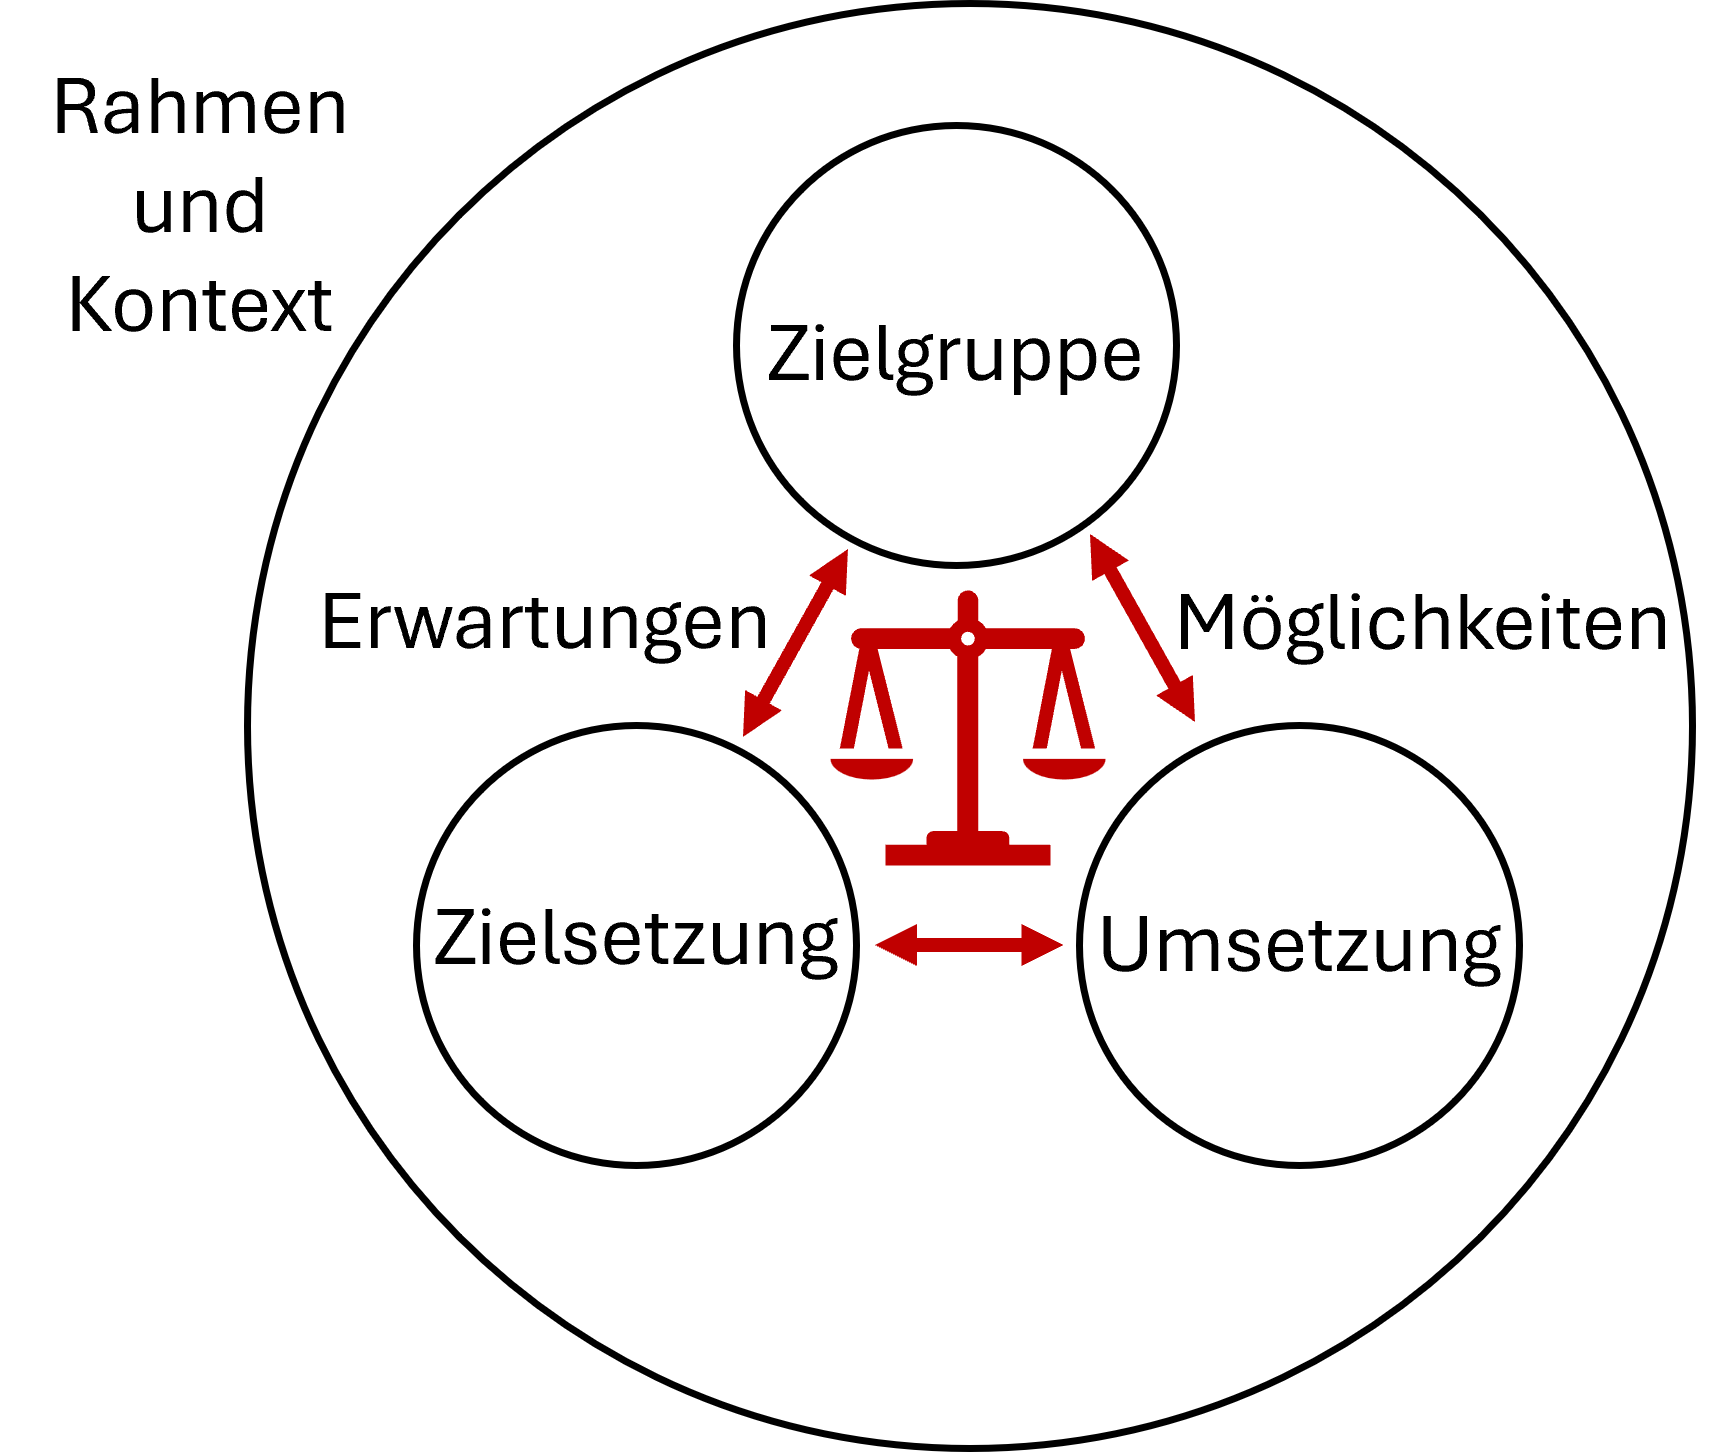
\includegraphics[width=\linewidth,height=.53\textheight,keepaspectratio]{images/kontext.png}
\end{frame}

\begin{frame}{Planung der Vortragsstruktur}
\begin{columns}[T,onlytextwidth]
  \column{.3\textwidth}
  \begin{myalert}[1 · Einstieg]
    Interesse wecken\\
    Vorwissen aktivieren\\
    Ziel und Ablauf klären
  \end{myalert}

  \column{.36\textwidth}
  \begin{mynote}[2 · Kernteil]
    Wenige klare Kernbotschaften\\
    Mit Beispielen und Bildern erklären\\
    Tiefe an die Zielgruppe anpassen\\
    Dem roten Faden folgen
  \end{mynote}

  \column{.3\textwidth}
  \begin{myalert}[3 · Schluss]
    Kernaussagen wiederholen\\
    Offene Fragen benennen\\
    Fazit und Ausblick geben
  \end{myalert}
\end{columns}
\end{frame}

\section{Design, Visualisierungen und Hilfsmittel}

\begin{frame}{Foliendesign}
\keyidea{Eine klare Aussage und eine passende Abbildung erleichtern die Orientierung.}
\vspace{2mm}
\begin{columns}[c,onlytextwidth]
  \column{.34\textwidth}
  \small
  \begin{itemize}
    \item Text auf das Wesentliche kürzen.
    \item Beschriftungen nahe am Bild platzieren.
    \item Kontraste und Freiraum nutzen.
    \item Lesbarkeit aus der letzten Reihe prüfen.
  \end{itemize}
  \column{.63\textwidth}
  \centering
  \resizebox{\linewidth}{!}{% Editable 16:9 slide example. Uses colors defined by LeipzigClean.
% Include inside a resizebox in main.tex. No external image is required.
\begin{tikzpicture}[x=1cm,y=1cm,font=\sffamily]
  \useasboundingbox (0,0) rectangle (12,6.75);
  \filldraw[fill=white,draw=Muted!45,line width=.6pt] (0,0) rectangle (12,6.75);
  \node[anchor=north west,text=Ink,font=\sffamily\bfseries\large,
        text width=10.9cm,inner sep=0pt] at (.5,6.25)
        {Am ebenen Spiegel sind Einfalls- und Reflexionswinkel gleich};
  % Left: short explanation; right: relevant figure with adjacent labels.
  \node[anchor=north west,text width=4.2cm,align=left,inner sep=0pt,
        font=\sffamily\normalsize] at (.5,4.65)
        {\textbf{Der Bezug ist das Lot.}\\[5mm]
         Beide Winkel werden zwischen Lichtstrahl und Lot gemessen.\\[6mm]
         \Large\textcolor{granat}{$\bm{\alpha}$} $\;\bm{=}\;$ \textcolor{LeipzigBlue}{$\quad\quad\bm{\beta}$}};
  \fill[aquamarin!20] (5.4,1.75) rectangle (11.45,1.97);
  \draw[Ink,line width=1.2pt] (5.4,1.97)--(11.45,1.97);
  \draw[dashed,Muted,line width=.8pt] (8.4,1.97)--(8.4,4.9);
  \node[anchor=south,font=\sffamily\small,text=Muted] at (8.4,4.95) {Lot};
  \draw[->,granat,line width=1.8pt,>=stealth] (5.9,4.47)--(8.4,1.97);
  \draw[->,LeipzigBlue,line width=1.8pt,>=stealth] (8.4,1.97)--(10.9,4.47);
  \draw[granat,line width=.9pt] (8.4,2.95) arc[start angle=90,end angle=135,radius=.98];
  \draw[LeipzigBlue,line width=.9pt] (9.093,2.663) arc[start angle=45,end angle=90,radius=.98];
  \node[text=granat,font=\large] at (7.91,3.23) {$\alpha$};
  \node[text=LeipzigBlue,font=\large] at (8.89,3.23) {$\beta$};
  \node[anchor=south east,font=\sffamily\small,text=granat] at (7.0,4.5) {einfallend};
  \node[anchor=south west,font=\sffamily\small,text=LeipzigBlue] at (9.8,4.5) {reflektiert};
  \node[anchor=north east,font=\sffamily\small,text=Muted] at (11.45,1.55) {ebener Spiegel};
  \draw[karneol,line width=.5pt] (.5,.68)--(11.5,.68);
  % \node[anchor=west,font=\sffamily\scriptsize,text=Muted] at (.5,.36)
       % {Schematische Darstellung};
\end{tikzpicture}
}
\end{columns}
\slidesource{Noetel et al. (2022)}
\note{Die Abbildung zeigt ein editierbares Layoutbeispiel, keine empirischen Daten.
Die Strahlenzeichnung bezieht sich auf Reflexion am ebenen Spiegel.
Wort- und Zeilenzahlen sind keine universellen, empirisch gesicherten Grenzwerte.
Auch Punktgrößen sind zwischen PowerPoint und Beamer nicht direkt übertragbar:
Die projizierte Lesbarkeit hängt von Folienformat, Raum und Betrachtungsabstand ab.
Für lernbezogene Gestaltungsprinzipien siehe \cite{noetel2022}.}
\end{frame}

\begin{frame}{Visualisierungen}

\keyalert{Was meint ihr: was macht eine gute Visualisierung aus?}

\vspace{3mm}
\begin{itemize}
  \item \textbf{Kohärenz:} Unnötige Details und dekorative Bilder weglassen.
  \item \textbf{Signalisierung:} Den entscheidenden Zusammenhang hervorheben.
  \item \textbf{Räumliche Nähe:} Bild und zugehörige Beschriftung zusammen zeigen.
  \item \textbf{Dosierung:} Komplexe Erklärungen in nachvollziehbare Schritte teilen.
\end{itemize}
\slidesource{Noetel et al. (2022); Fiorella \& Mayer (2021)}
\note{\cite{noetel2022,fiorella2021}. Die Evidenz betrifft überwiegend Lernen mit
multimedialen Materialien. Daraus folgt kein universelles Rezept für jede Rede.
Zum Beispiel jeweils den besprochenen Lichtstrahl hervorheben. Zugänglichkeit und
sprachliche Voraussetzungen bei der Entscheidung über sichtbaren Text berücksichtigen.}
\end{frame}

\begin{frame}{Hilfsmittel}
\begin{columns}[c,onlytextwidth]
  \column{.43\textwidth}
  \small
  \begin{itemize}
    \item Folien, Handouts, Flipcharts, Whiteboards, Overheadprojektoren
    \item Modelle, Anschauungsmaterial, Experimente
    \item Videos, Animationen, Simulationen
    \item Quizze, Umfragen, Abstimmungen: Lernen während des Vortrags.
  \end{itemize}
  \column{.54\textwidth}
  \centering
  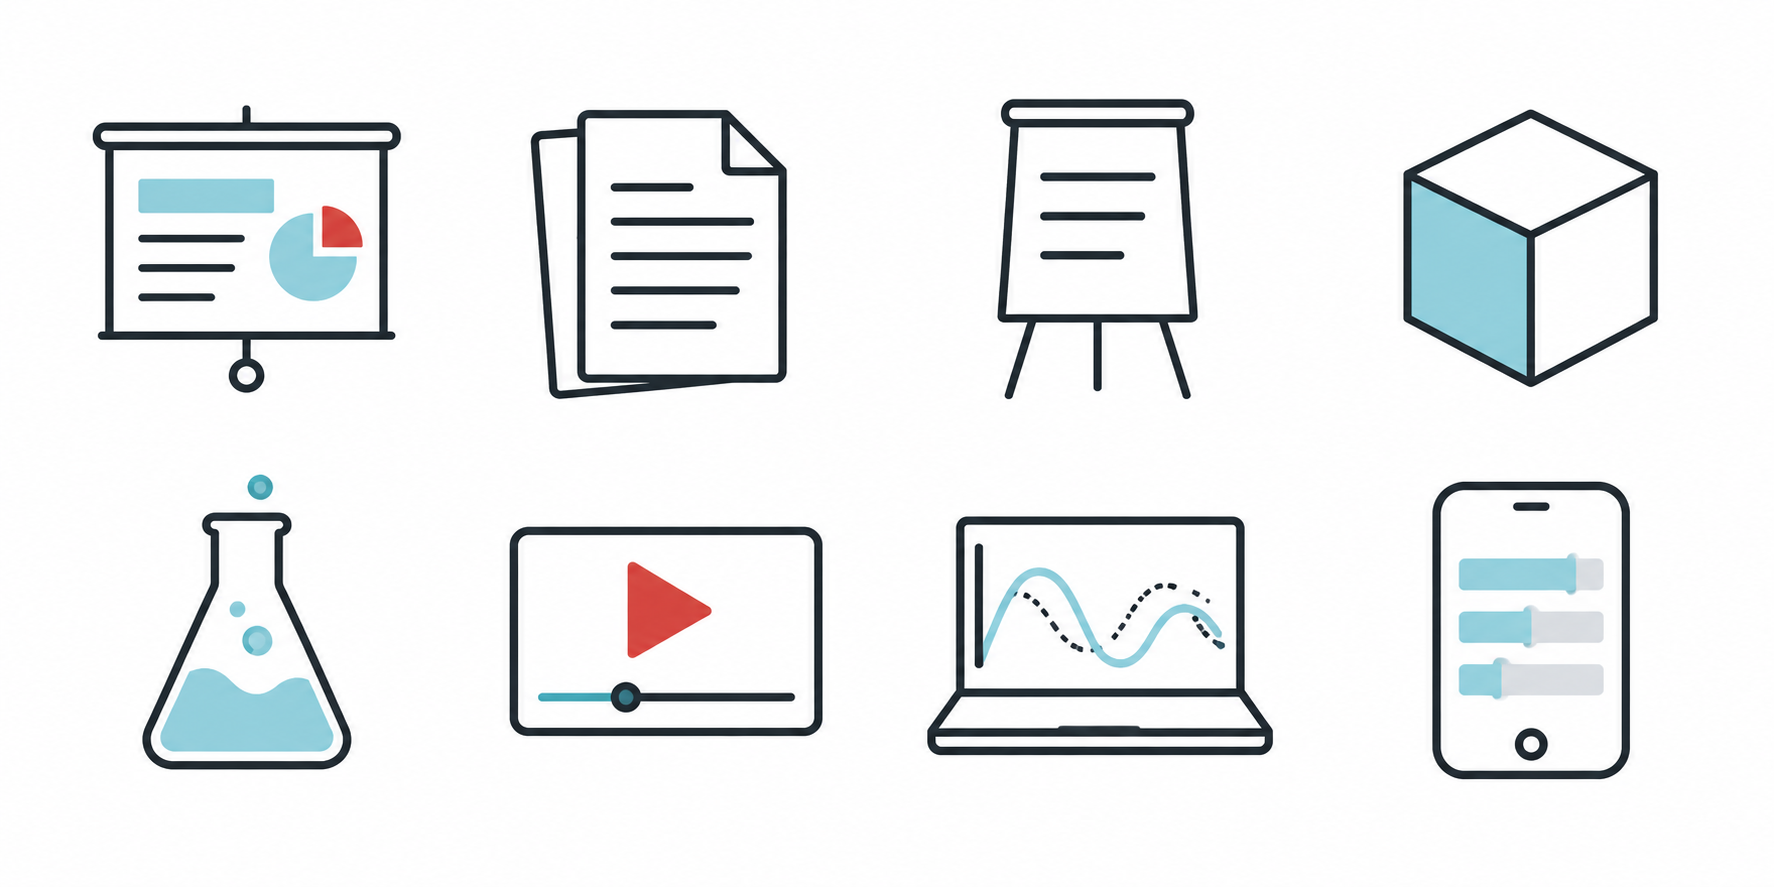
\includegraphics[width=\linewidth]{images/hilfsmittel-icons.png}
\end{columns}
\vspace{4mm}
\keyidea{Was können die Zuhörenden damit besser verstehen oder selbst erarbeiten?}
\note{Iconübersicht: Folien, Handout, Flipchart, Modell, Experiment, Video,
Simulation und Umfrage. KI-generierte Illustration mit dem integrierten Bildwerkzeug,
7. Oktober 2026. Die Bildzeichen dienen der Zuordnung der Beispiele.}
\end{frame}

\section{Mündliche Präsentationen halten}
\begin{frame}{Mündliche Präsentationen halten}
\keyidea{Du bist die Präsentation, nicht die Folien.}
\vspace{3mm}
\footnotesize
Natürliche und effektive Kommunikation bedeutet ...

\begin{mynote}[... Verbal]
  \begin{itemize}
    \item die Inhalte klar und verständlich zu vermitteln,
    \item die Aufmerksamkeit der Zuhörer*innen zu halten,
    \item die Botschaften zu betonen und zu verstärken.
  \end{itemize}
\end{mynote}

\begin{mynote}[... Nonverbal]
  \begin{itemize}
    \item Körpersprache, Gestik, Mimik und Blickkontakt bewusst einsetzen,
    \item Stimme, Lautstärke, Sprechtempo und Pausen variieren,
    \item Raum und Hilfsmittel effektiv nutzen.
  \end{itemize}
\end{mynote}
\end{frame}

\section{Beispiel aus der Optik}

\begin{frame}{Beispiel aus der Optik}
  \centering
  \keyalert{Plant einen Vortrag zum Thema Optik anhand des Handouts für eure Mitstudierenden.}
  \begin{columns}
    \column{0.5\textwidth}
    Überlegt euch
    \begin{itemize}
    \item Ziel und Struktur des Vortrags,
    \item Kernbotschaften für den Unterricht,
    \item Visualisierung, die die Kernbotschaften oder einen Teil davon unterstützt,
    \item Methoden und Materialien, die ihr einsetzen würdet.
    \end{itemize}
    \column{0.5\textwidth}
    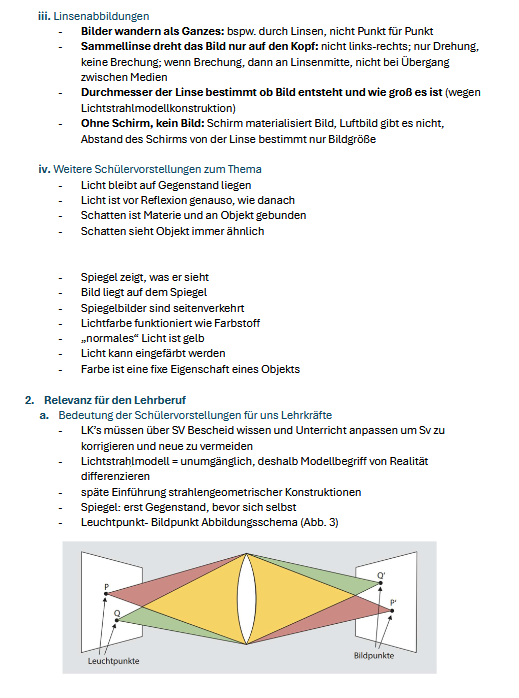
\includegraphics[width=0.6\textwidth]{images/optik_handout.png}
  \end{columns}

\end{frame}

\section{Feedback im Lehrberuf}
\begin{frame}{Relevanz von Feedback für den Lehrberuf}
\keyidea{Feedback kann Lernen unterstützen. Sein Informationsgehalt ist entscheidend.}
\vspace{4mm}
435 Studien zeigen im Mittel $d=0{,}48$ \citep{10.3389/fpsyg.2019.03087}
\vspace{4mm}

23 Studien: kleine mittlere Verbesserung der Unterrichtsqualität $d=0{,}27$ \citep{roehl2025}

Größere Effekte bei 
\begin{itemize}
  \item Unterstützung der Interpretation,
  \item Dialog mit der Klasse,
  \item Möglichkeit, Feedback umzusetzen. 
\end{itemize}

% \source{$d$ bezeichnet eine standardisierte Effektgröße, keinen prozentualen Lernzuwachs.}
% \slidesource{Wisniewski et al. (2020); Brandmo \& Gamlem (2025)}
\note{\cite{10.3389/fpsyg.2019.03087,brandmo2025}.
In Tabelle 3 der Metaanalyse stehen für Lehrende an Lernende d=.47 und für
Peers d=.85, bei sehr ungleichen Teilgruppen (812 bzw. 16 Effekte).
Diese Vergleiche zwischen Studien erlauben keine kausale Rangfolge der Feedbackgeber.
Auch d=.99 für hochinformatives Feedback ist ein heterogener Teilgruppenbefund,
kein garantierter Effekt. Brandmo und Gamlem betrachten 96 Studien zu 10- bis
16-Jährigen mit unterschiedlichen Designs, darunter viele Beobachtungsstudien.}
\end{frame}

\begin{frame}{Feedback geben}
\keyidea{Feedback sollte informativ, zugeschnitten, und handlungsorientiert sein \citep{brandmo2025}. }
\vspace{3mm}

\begin{itemize}
  \item Beobachten, nicht bewerten, zum Beispiel \glqq Auf Folie X hast du das Thema von Argument Y bis zu Argument Z aufgearbeitet\grqq.
  \item Wirkung auf die eigene Person beschreiben, zum Beispiel \glqq Für mich war das schwer verständlich, schwierig nachzuvollziehen\grqq.
  \item Handlungsorientiert sein, zum Beispiel \glqq Du könntest das Argument Z noch mit einem Beispiel untermauern  oder die Argumentation mit einem Flussdiagramm beschreiben\grqq.
  \item Negativität und Schwammigkeit vermeiden.
  \item Bereit sein, Rückfragen zu beantworten.
\end{itemize}

% \slidesource{Wisniewski et al. (2020); Brandmo \& Gamlem (2025)}
\note{\cite{10.3389/fpsyg.2019.03087,brandmo2025}. Das Beispiel ist selbst
formuliert. Ein respektvoller Rahmen bleibt wichtig. Sofortiges Feedback ist
nicht für jede Aufgabe grundsätzlich besser als verzögertes Feedback.}
\end{frame}

\begin{frame}{Feedback annehmen}
\keyidea{Feedback nutzen heißt verstehen, abwägen und eine Verbesserung erproben.}
\vspace{3mm}
\begin{itemize}
  \item \textbf{Aktiv Zuhören:} Die Rückmeldung zunächst vollständig aufnehmen und zum Beispiel paraphrasieren.
  \item \textbf{Nachfragen:} Zum Beispiel um ein konkretes Beispiel oder die zugrunde liegenden Schwierigkeiten genauer erfragen.
  \item \textbf{Abwägen:} Die Rückmeldung mit dem Lernziel und der eigenen Beobachtung vergleichen.
  \item \textbf{Umsetzen:} Mögliche nächste Schritte beschreiben und Rückmeldung dazu einholen.
\end{itemize}

\keyalert{Wir probieren es aus: Findet euch mit einem anderen Paar zusammen, zeigt euren Plan zum Optikvortrag und lasst euch Feedback geben.}

\note{Die Regeln sind eine praktische Ableitung aus der Forschung zur
Feedbackaufnahme \cite{brandmo2025}, kein empirisch geprüftes Regelpaket.}
\end{frame}

\section{Feedbackmethoden}
\begin{frame}{Feedbackmethoden 1}
\footnotesize
\begin{mynote}[5-Finger-Feedback]
Die SuS malen die Umrisse ihrer Hand auf ein Blatt Papier. An jeden Finger schreiben sie eine
Bemerkung zum Kurs/zum Thema:
\begin{itemize}
  \item An den Daumen schreiben sie etwas, das sie weiterverfolgen wollen „Da halte
ich den Daumen drauf“ (Alternativ: Thumbs up – „das fand ich super“)
\item Zeigefinger: „Das habe ich gelernt, das will ich mir merken“
\item Mittelfinger: „Das hat mir gestunken“
\item Ringfinger: „Die Atmosphäre hier…“
\item Kleiner Finger: „Folgendes ist mir zu kurz gekommen…“
\end{itemize}
\end{mynote}
\end{frame}

\begin{frame}{Feedbackmethoden 2}
  \footnotesize
\begin{mynote}[Blitzlicht]
ein oder zwei Fragen formulieren (am besten verschriftlichen), z.B.:
\begin{itemize}
\item Was war das Wichtigste, das ich heute gelernt habe?
\item Was hätte ich gerne anders gehabt?
\item Was hätte ich gerne zusätzlich gehabt?/Was brauche ich noch?
\end{itemize} 
SuS antworten ganz knapp darauf
Regeln: Kurz (ca. 2-3 Sätze); Konkret; kein Kommentar/keine Diskussion
\end{mynote}
\footnotesize
\begin{mynote}[Mentimeter]
Feedback kann auch digital über Mentimeter gesammelt werden. Die SuS geben ihre Rückmeldungen anonym ein, und die Ergebnisse werden in Echtzeit visualisiert. Fragen können z.B. sein: "Was hat dir besonders gefallen?" oder "Was könnte ich verbessern?"
\end{mynote}

\end{frame}

\begin{frame}{Feedbackmethoden 3}
\footnotesize
  \begin{mynote}[Feedbackanker]
Verschiedene Aspekte, zu denen Feedback gegeben werden soll, werden mit je einer Farbe
versehen: Inhalt, Struktur, Körpersprache, Stimme und Sprache etc.

SuS erhalten vor dem Vortrag einen kleinen Zettel in einer der Farben. Sie müssen sich
nun während des Beitrags nur auf die eigene Kategorie konzentrieren und dazu Feedback geben. 
So erhalten die Vortragenden hinterher ein umfassendes Feedback.
  \end{mynote}
  \begin{mynote}[Interaktive Mindmap]
    In einer interaktiven Mindmap kann Feedback zu verschiedenen Aspekten einer Präsentation gesammelt werden. Die SuS tragen ihre Rückmeldungen zu den einzelnen Kategorien in die Mindmap ein, sodass ein umfassendes Bild entsteht. Kategorien könnten sein: Inhalt, Struktur, Visualisierung und Verständlichkeit. 
  \end{mynote}
\end{frame}

\begin{frame}{Feedbackmethoden 4}
  \footnotesize
\begin{mynote}[One-Minute-Paper]
  Die SuS sollen kurz schriftlich eine Frage beantworten.
Dazu werden Karten ausgeteilt, die vorne mit einem Minus, hinten mit einem Plus markiert sind.
(Alternativ werden die Teilnehmer gebeten, ein Blatt zu halbieren und selbst zu markieren).
Auf die Vorderseite sollen sie dann schreiben, was ihnen an der Veranstaltung besonders gefallen
hat, auf die Rückseite was sie sich im weiteren Verlauf an Veränderungen wünschen.
Die Art der Fragestellung bestimmt mit, wie präzise die Antworten sind. Logischerweise können mit
unterschiedlichen Fragen unterschiedliche Ziele verfolgt werden.
Alternative Fragen:
\begin{itemize}
\item Was war für Dich heute der Kernpunkt des Vortrags?
\item Was war die Hauptfrage, die für Dich heute unbeantwortet blieb?
\item Was ist für Dich die wichtigste Einsicht, die Du aus dieser Kurseinheit/Diskussion mitnimmst?
\item Welches Argument hat Dich nicht überzeugt?
\end{itemize}
\end{mynote}
\end{frame}


\section{Abschluss und Fazit}
\begin{frame}{Abschluss und Fazit}
\begin{itemize}
  \item Die Planung von Präsentationen sollte das Wechselspiel zwischen Zielgruppe, Zielsetzung und Umsetzung im Kontext berücksichtigen.
  \item Eine klare Strategie und Struktur ist entscheidend für eine erfolgreiche Präsentation.
  \item Visualisierungen und Hilfsmittel sollten die Präsentation unterstützen, nicht ersetzen.
  \item \textit{Du} bist die Präsentation, nicht die Folien: verbale und nonverbale Kommunikation beachten.
  \item Gutes Feedback ist ein wertvolles Geschenk.
\end{itemize}

Ausblick: Ihr haltet im Semester fachliche Vorträge. Informationsblatt beachten. Überlegt euch zudem eine Feedbackmethode und wendet sie an.
\end{frame}

\begin{frame}{Literatur: Präsentationen}
  \footnotesize
  \nocite{noetel2022,fiorella2021,agarwal2021,10.3389/fpsyg.2019.03087,brandmo2025,roehl2025,levinielsen2026}
  \printbibliography[heading=none,keyword=presentation]
\end{frame}

\begin{frame}{Literatur: Feedback}
  \footnotesize
  \printbibliography[heading=none,keyword=learningfeedback]
\end{frame}

\appendix
\section{Example layouts}

\end{document}
